\documentclass[a4paper]{article}

\usepackage[margin=1.5cm]{geometry}
\usepackage{tikz}
\usetikzlibrary{calc}
\usepackage{xcolor}

\pagestyle{empty}

\begin{document}

\begin{center}
  \begin{tabular}{cccc}
    % 25°
    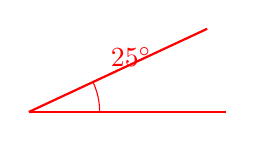
\begin{tikzpicture}[scale=1]
      \color{red}
      \coordinate (O) at (0,0);
      \draw[thick] (O) -- ++(2.5,0);
      \draw[thick] (O) -- ++(25:2.5);
      \draw (O) ++(0.9,0) arc (0:25:0.9);
      \node at ($(O)+(1.3,0.7)$) {$25^\circ$};
    \end{tikzpicture}
    &
    % 30°
    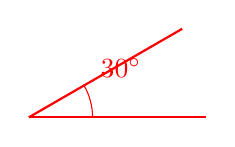
\begin{tikzpicture}[scale=0.9]
      \color{red}
      \coordinate (O) at (0,0);
      \draw[thick] (O) -- ++(2.5,0);
      \draw[thick] (O) -- ++(30:2.5);
      \draw (O) ++(0.9,0) arc (0:30:0.9);
      \node at ($(O)+(1.3,0.7)$) {$30^\circ$};
    \end{tikzpicture}
    &
    % 40°
    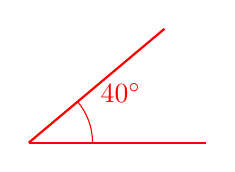
\begin{tikzpicture}[scale=0.9]
      \color{red}
      \coordinate (O) at (0,0);
      \draw[thick] (O) -- ++(2.5,0);
      \draw[thick] (O) -- ++(40:2.5);
      \draw (O) ++(0.9,0) arc (0:40:0.9);
      \node at ($(O)+(1.3,0.7)$) {$40^\circ$};
    \end{tikzpicture}
    &
    % 45°
    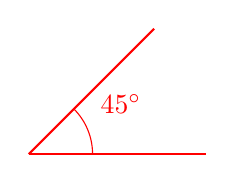
\begin{tikzpicture}[scale=0.9]
      \color{red}
      \coordinate (O) at (0,0);
      \draw[thick] (O) -- ++(2.5,0);
      \draw[thick] (O) -- ++(45:2.5);
      \draw (O) ++(0.9,0) arc (0:45:0.9);
      \node at ($(O)+(1.3,0.7)$) {$45^\circ$};
    \end{tikzpicture}
    \\[0.4em]
    % 55°
    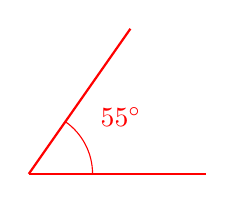
\begin{tikzpicture}[scale=0.9]
      \color{red}
      \coordinate (O) at (0,0);
      \draw[thick] (O) -- ++(2.5,0);
      \draw[thick] (O) -- ++(55:2.5);
      \draw (O) ++(0.9,0) arc (0:55:0.9);
      \node at ($(O)+(1.3,0.8)$) {$55^\circ$};
    \end{tikzpicture}
    &
    % 70°
    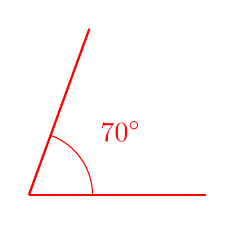
\begin{tikzpicture}[scale=0.9]
      \color{red}
      \coordinate (O) at (0,0);
      \draw[thick] (O) -- ++(2.5,0);
      \draw[thick] (O) -- ++(70:2.5);
      \draw (O) ++(0.9,0) arc (0:70:0.9);
      \node at ($(O)+(1.3,0.9)$) {$70^\circ$};
    \end{tikzpicture}
    &
    % 80°
    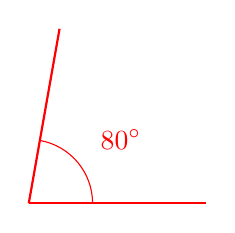
\begin{tikzpicture}[scale=0.9]
      \color{red}
      \coordinate (O) at (0,0);
      \draw[thick] (O) -- ++(2.5,0);
      \draw[thick] (O) -- ++(80:2.5);
      \draw (O) ++(0.9,0) arc (0:80:0.9);
      \node at ($(O)+(1.3,0.9)$) {$80^\circ$};
    \end{tikzpicture}
    &
    % 100°
    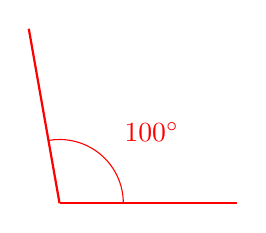
\begin{tikzpicture}[scale=0.9]
      \color{red}
      \coordinate (O) at (0,0);
      \draw[thick] (O) -- ++(2.5,0);
      \draw[thick] (O) -- ++(100:2.5);
      \draw (O) ++(0.9,0) arc (0:100:0.9);
      \node at ($(O)+(1.3,1.0)$) {$100^\circ$};
    \end{tikzpicture}
    \\[0.4em]
    % 120°
    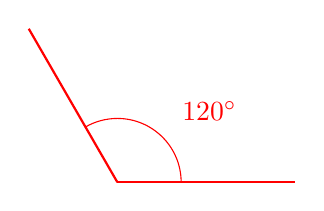
\begin{tikzpicture}[scale=0.9]
      \color{red}
      \coordinate (O) at (0,0);
      \draw[thick] (O) -- ++(2.5,0);
      \draw[thick] (O) -- ++(120:2.5);
      \draw (O) ++(0.9,0) arc (0:120:0.9);
      \node at ($(O)+(1.3,1.0)$) {$120^\circ$};
    \end{tikzpicture}
    &
    % 135°
    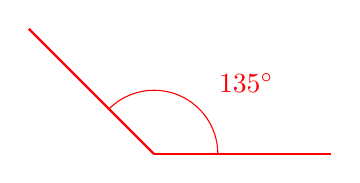
\begin{tikzpicture}[scale=0.9]
      \color{red}
      \coordinate (O) at (0,0);
      \draw[thick] (O) -- ++(2.5,0);
      \draw[thick] (O) -- ++(135:2.5);
      \draw (O) ++(0.9,0) arc (0:135:0.9);
      \node at ($(O)+(1.3,1.0)$) {$135^\circ$};
    \end{tikzpicture}
    &
    % 140°
    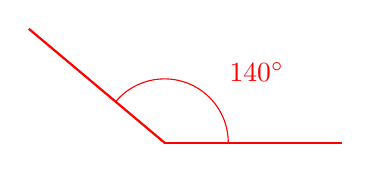
\begin{tikzpicture}[scale=0.9]
      \color{red}
      \coordinate (O) at (0,0);
      \draw[thick] (O) -- ++(2.5,0);
      \draw[thick] (O) -- ++(140:2.5);
      \draw (O) ++(0.9,0) arc (0:140:0.9);
      \node at ($(O)+(1.3,1.0)$) {$140^\circ$};
    \end{tikzpicture}
    &
    % 160°
    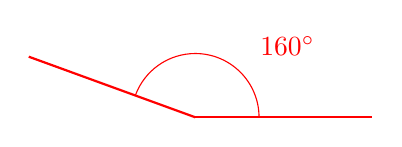
\begin{tikzpicture}[scale=0.9]
      \color{red}
      \coordinate (O) at (0,0);
      \draw[thick] (O) -- ++(2.5,0);
      \draw[thick] (O) -- ++(160:2.5);
      \draw (O) ++(0.9,0) arc (0:160:0.9);
      \node at ($(O)+(1.3,1.0)$) {$160^\circ$};
    \end{tikzpicture}
    \\[0.4em]
    % 255°
    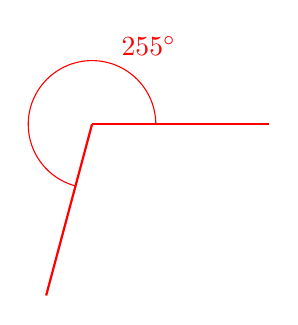
\begin{tikzpicture}[scale=0.9]
      \color{red}
      \coordinate (O) at (0,0);
      \draw[thick] (O) -- ++(2.5,0);
      \draw[thick] (O) -- ++(255:2.5);
      \draw (O) ++(0.9,0) arc (0:255:0.9);
      \node at ($(O)+(0.8,1.1)$) {$255^\circ$};
    \end{tikzpicture}
    &
    % 260°
    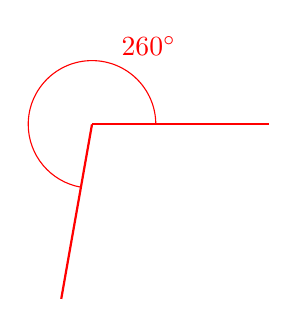
\begin{tikzpicture}[scale=0.9]
      \color{red}
      \coordinate (O) at (0,0);
      \draw[thick] (O) -- ++(2.5,0);
      \draw[thick] (O) -- ++(260:2.5);
      \draw (O) ++(0.9,0) arc (0:260:0.9);
      \node at ($(O)+(0.8,1.1)$) {$260^\circ$};
    \end{tikzpicture}
    &
    % 265°
    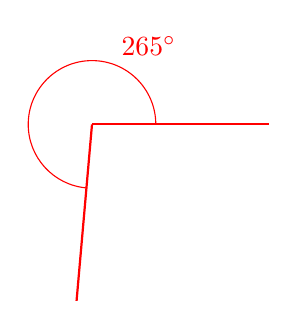
\begin{tikzpicture}[scale=0.9]
      \color{red}
      \coordinate (O) at (0,0);
      \draw[thick] (O) -- ++(2.5,0);
      \draw[thick] (O) -- ++(265:2.5);
      \draw (O) ++(0.9,0) arc (0:265:0.9);
      \node at ($(O)+(0.8,1.1)$) {$265^\circ$};
    \end{tikzpicture}
    &
    % 270°
    \begin{tikzpicture}[scale=0.9]
      \color{red}
      \coordinate (O) at (0,0);
      \draw[thick] (O) -- ++(2.5,0);
      \draw[thick] (O) -- ++(270:2.5);
      \draw (O) ++(0.9,0) arc (0:270:0.9);
      \node at ($(O)+(0.8,1.1)$) {$270^\circ$};
    \end{tikzpicture}
    \\[0.4em]
    % 290°
    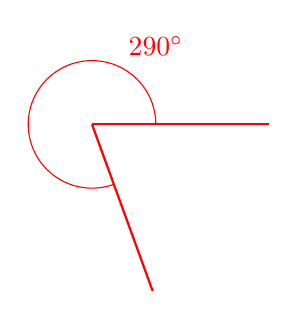
\begin{tikzpicture}[scale=0.9]
      \color{red}
      \coordinate (O) at (0,0);
      \draw[thick] (O) -- ++(2.5,0);
      \draw[thick] (O) -- ++(290:2.5);
      \draw (O) ++(0.9,0) arc (0:290:0.9);
      \node at ($(O)+(0.9,1.1)$) {$290^\circ$};
    \end{tikzpicture}
    &
    % 300°
    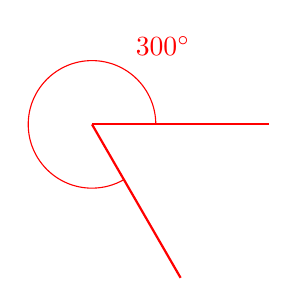
\begin{tikzpicture}[scale=0.9]
      \color{red}
      \coordinate (O) at (0,0);
      \draw[thick] (O) -- ++(2.5,0);
      \draw[thick] (O) -- ++(300:2.5);
      \draw (O) ++(0.9,0) arc (0:300:0.9);
      \node at ($(O)+(1.0,1.1)$) {$300^\circ$};
    \end{tikzpicture}
    &
    % 315°
    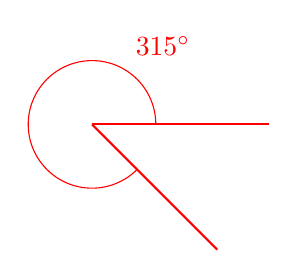
\begin{tikzpicture}[scale=0.9]
      \color{red}
      \coordinate (O) at (0,0);
      \draw[thick] (O) -- ++(2.5,0);
      \draw[thick] (O) -- ++(315:2.5);
      \draw (O) ++(0.9,0) arc (0:315:0.9);
      \node at ($(O)+(1.0,1.1)$) {$315^\circ$};
    \end{tikzpicture}
    &
    % empty cell (no 20th angle)
    {}
  \end{tabular}
\end{center}

\vspace{0.3em}

\begin{center}
  \begin{tabular}{cc}
    % Q3 - Version A
    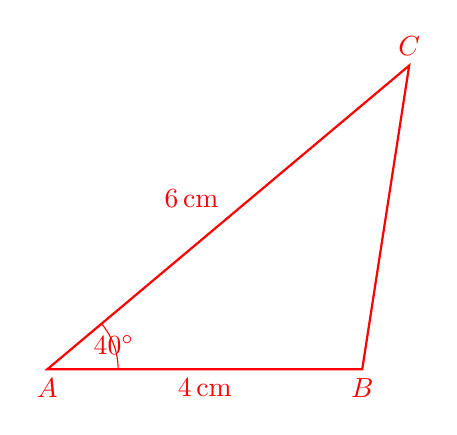
\begin{tikzpicture}[scale=1]
      \color{red}
      \def\AB{4}
      \def\AC{6}
      \def\ang{40}

      \coordinate (A) at (0,0);
      \coordinate (B) at (\AB,0);
      \coordinate (C) at ({\AC*cos(\ang)},{\AC*sin(\ang)});

      \draw[thick] (A) -- (B) -- (C) -- cycle;
      \draw (A) ++(0.9,0) arc (0:\ang:0.9);

      % Mesures
      \node[below] at ($(A)!0.5!(B)$) {$\AB\,\mathrm{cm}$};
      \node[above left] at ($(A)!0.5!(C)$) {$\AC\,\mathrm{cm}$};
      \node at ({0.9*cos(\ang/2)},{0.9*sin(\ang/2)}) {$\ang^\circ$};

      % Sommets
      \node[below] at (A) {$A$};
      \node[below] at (B) {$B$};
      \node[above] at (C) {$C$};
    \end{tikzpicture}
    &
    % Q3 - Version B
    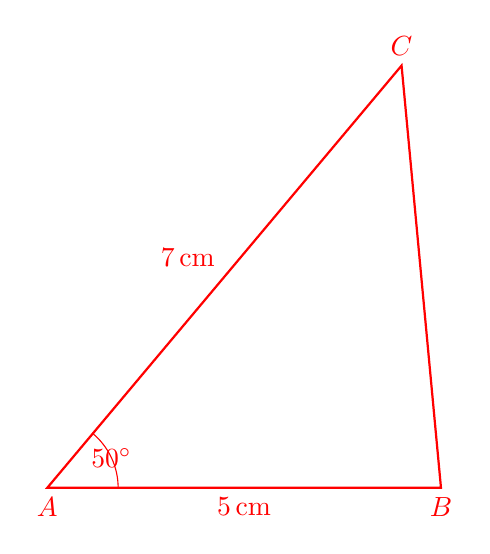
\begin{tikzpicture}[scale=1]
      \color{red}
      \def\AB{5}
      \def\AC{7}
      \def\ang{50}

      \coordinate (A) at (0,0);
      \coordinate (B) at (\AB,0);
      \coordinate (C) at ({\AC*cos(\ang)},{\AC*sin(\ang)});

      \draw[thick] (A) -- (B) -- (C) -- cycle;
      \draw (A) ++(0.9,0) arc (0:\ang:0.9);

      % Mesures
      \node[below] at ($(A)!0.5!(B)$) {$\AB\,\mathrm{cm}$};
      \node[above left] at ($(A)!0.5!(C)$) {$\AC\,\mathrm{cm}$};
      \node at ({0.9*cos(\ang/2)},{0.9*sin(\ang/2)}) {$\ang^\circ$};

      % Sommets
      \node[below] at (A) {$A$};
      \node[below] at (B) {$B$};
      \node[above] at (C) {$C$};
    \end{tikzpicture}
    \\
    % Q3 - Version C
    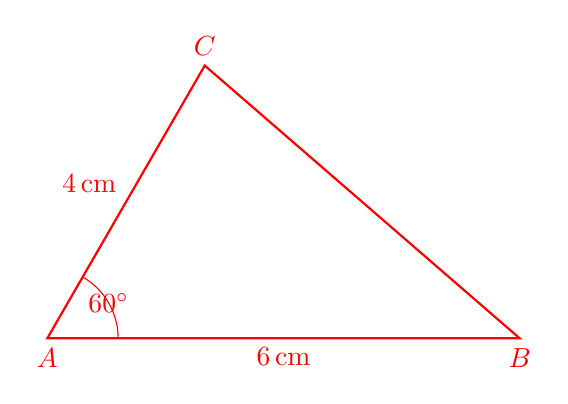
\begin{tikzpicture}[scale=1]
      \color{red}
      \def\AB{6}
      \def\AC{4}
      \def\ang{60}

      \coordinate (A) at (0,0);
      \coordinate (B) at (\AB,0);
      \coordinate (C) at ({\AC*cos(\ang)},{\AC*sin(\ang)});

      \draw[thick] (A) -- (B) -- (C) -- cycle;
      \draw (A) ++(0.9,0) arc (0:\ang:0.9);

      % Mesures
      \node[below] at ($(A)!0.5!(B)$) {$\AB\,\mathrm{cm}$};
      \node[above left] at ($(A)!0.5!(C)$) {$\AC\,\mathrm{cm}$};
      \node at ({0.9*cos(\ang/2)},{0.9*sin(\ang/2)}) {$\ang^\circ$};

      % Sommets
      \node[below] at (A) {$A$};
      \node[below] at (B) {$B$};
      \node[above] at (C) {$C$};
    \end{tikzpicture}
    &
    % Q3 - Version D
    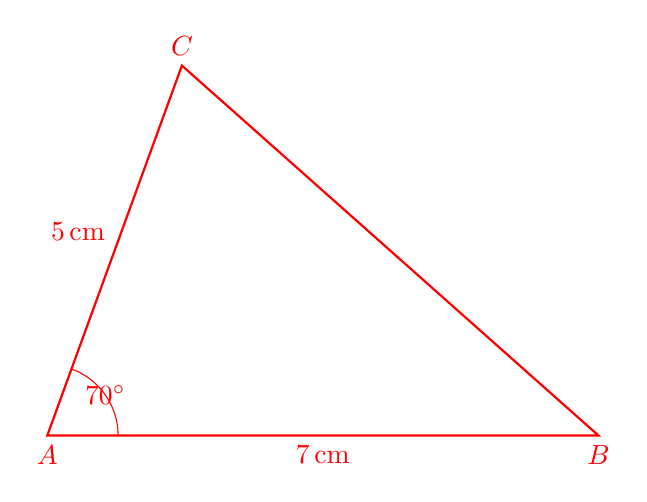
\begin{tikzpicture}[scale=1]
      \color{red}
      \def\AB{7}
      \def\AC{5}
      \def\ang{70}

      \coordinate (A) at (0,0);
      \coordinate (B) at (\AB,0);
      \coordinate (C) at ({\AC*cos(\ang)},{\AC*sin(\ang)});

      \draw[thick] (A) -- (B) -- (C) -- cycle;
      \draw (A) ++(0.9,0) arc (0:\ang:0.9);

      % Mesures
      \node[below] at ($(A)!0.5!(B)$) {$\AB\,\mathrm{cm}$};
      \node[above left] at ($(A)!0.5!(C)$) {$\AC\,\mathrm{cm}$};
      \node at ({0.9*cos(\ang/2)},{0.9*sin(\ang/2)}) {$\ang^\circ$};

      % Sommets
      \node[below] at (A) {$A$};
      \node[below] at (B) {$B$};
      \node[above] at (C) {$C$};
    \end{tikzpicture}
  \end{tabular}
\end{center}

\end{document}
